\chapter{Appendix}

\section{Shell}

A shell is actually how you are going to be interacting with the system. Before user-friendly operating systems, when a computer started up all you had access to was a shell. This meant that all of your commands and editing had to be done this way. Nowadays, our computers boot up in desktop mode, but one can still access a shell using a terminal.

\begin{lstlisting}[language=bash]
(Stuff) $
\end{lstlisting}

It is ready for your next command! You can type in a lot of Unix utilities like \keyword{ls}, \keyword{echo\ Hello} and the shell will execute them and give you the result. Some of these are what are known as \keyword{shell-builtins} meaning that the code is in the shell program itself. Some of these are compiled programs that you run. The shell only looks through a special variable called path which contains a list of colon separated paths to search for an executable with your name, here is an example path.

\begin{lstlisting}[language=bash]
$ echo $PATH
/usr/local/sbin:/usr/local/bin:/usr/sbin:
/usr/bin:/sbin:/bin:/usr/games:/usr/local/games
\end{lstlisting}

So when the shell executes \keyword{ls}, it looks through all of those directories, finds \keyword{/bin/ls} and executes that.

\begin{lstlisting}[language=bash]
$ ls
...
$ /bin/ls
\end{lstlisting}

You can always call through the full path. That is always why in past classes if you want to run something on the terminal you've had to do \keyword{./exe} because typically the directory that you are working in is not in the \keyword{PATH} variable. The \keyword{.} expands to your current directory and your shell executes \keyword{\textless{}current\_dir\textgreater{}/exe} which is a valid command.

\subsection{Shell tricks and tips}

\begin{itemize}
\item The up arrow will get you your most recent command
\item \keyword{ctrl-r} will search commands that you previously ran
\item \keyword{ctrl-c} will interrupt your shell's process
\item \keyword{!!} will execute the last command
\item \keyword{!<num>} goes back that many commands and runs that
\item \keyword{!<prefix>} runs the last command that has that prefix
\item \keyword{!\$} is the last arg of the previous command
\item \keyword{!*} is all args of the previous command
\item \keyword{\^pat\^sub} takes the last command and substitutes the pattern pat for the substitution sub
\item \keyword{cd -} goes to the previous directory
\item \keyword{pushd <dir>} pushes the current directory on a stack and cds
\item \keyword{popd} cds to the directory at the top of the stack
\end{itemize}

\subsection{What's a terminal?}

A terminal is an application that displays the output from the shell. You can have your default terminal, a quake based terminal, terminator, the options are endless!

\subsection{Common Utilities}

\begin{enumerate}
\item \keyword{cat} concatenate multiple files. It is regularly used to print out the contents of a file to the terminal but the original use was concatenation.

\begin{lstlisting}[language=bash]
$ cat file.txt
...
$ cat shakespeare.txt shakespeare.txt > two_shakes.txt
\end{lstlisting}

\item \keyword{diff} tells you the difference between the two files. If nothing is printed, then zero is returned meaning the files are the same byte for byte. Otherwise, the longest common subsequence difference is printed

\begin{lstlisting}[language=bash]
$ cat prog.txt
hello
world
$ cat adele.txt
hello
it's me
$ diff prog.txt prog.txt
$ diff shakespeare.txt shakespeare.txt
2c2
< world
---
> it's me
\end{lstlisting}

\item \keyword{grep} tells you which lines in a file or standard input match a POSIX pattern.

\begin{lstlisting}[language=bash]
$ grep it adele.txt
it's me
\end{lstlisting}

\item \keyword{ls} tells you which files are in the current directory.
\item \keyword{cd} this is a shell builtin but it changes to a relative or absolute directory

\begin{lstlisting}[language=bash]
$ cd /usr
$ cd lib/
$ cd -
$ pwd
/usr/
\end{lstlisting}

\item \keyword{man} every system programmers favorite command tells you more about all your favorite functions!
\item \keyword{make} executes programs according to a makefile.

\end{enumerate}

\subsection{Syntactic}

Shells have many useful utilities like saving some output to a file using redirection \keyword{>}.
This overwrites the file from the beginning.
If you only meant to append to the file, you can use \keyword{>>}.
Unix also allows file descriptor swapping.
This means that you can take the output going to one file descriptor and make it seem like it's coming out of another.
The most common one is \keyword{2>&1} which means take the stderr and make it seem like it is coming out of standard out.
This is important because when you use \keyword{>} and \keyword{>>} they only write the standard output of the file.
There are some examples below.

\begin{lstlisting}[language=bash]
$ ./program > output.txt # To overwrite
$ ./program >> output.txt # To append
$ ./program 2>&1 > output_all.txt # stderr & stdout
$ ./program 2>&1 > /dev/null # don't care about any output
\end{lstlisting}

The pipe operator has a fascinating history.
The UNIX philosophy is writing small programs and chaining them together to do new and interesting things.
Back in the early days, hard disk space was limited and write times were slow.
Brian Kernighan wanted to maintain the philosophy while omitting intermediate files that take up hard drive space.
So, the UNIX pipe was born.
A pipe takes the \keyword{stdout} of the program on its left and feeds it to the \keyword{stdin} of the program on its write.
Consider the command \keyword{tee}.
It can be used as a replacement for the redirection operators because tee will both write to a file and output to standard out.
It also has the added benefit that it doesn't need to be the last command in the list. Meaning, that you can write an intermediate result and continue your piping.

\begin{lstlisting}[language=bash]
$ ./program | tee output.txt # Overwrite
$ ./program | tee -a output.txt # Append
$ head output.txt | wc | head -n 1 # Multi pipes
$ ((head output.txt) | wc) | head -n 1 # Same as above
$ ./program | tee intermediate.txt | wc
\end{lstlisting}

The \keyword{&&} and \keyword{||} operator are operators that execute a command sequentially. \keyword{&&} only executes a command if the previous command succeeds, and \keyword{||} always executes the next command.

\begin{lstlisting}[language=bash]
$ false && echo "Hello!"
$ true && echo "Hello!"
$ false || echo "Hello!"
\end{lstlisting}

\subsection{What are environment variables?}

Each process gets its own dictionary of environment variables that are copied over to the child. Meaning, if the parent changes their environment variables it won't be transferred to the child and vice versa. This is important in the fork-exec-wait trilogy if you want to exec a program with different environment variables than your parent (or any other process).

For example, you can write a C program that loops through all of the time zones and executes the \keyword{date} command to print out the date and time in all locals. Environment variables are used for all sorts of programs so modifying them is important.


\subsubsection{Struct packing}

Structs may require something called \href{http://www.catb.org/esr/structure-packing/}{padding} (tutorial).
\textbf{We do not expect you to pack structs in this course, know that compilers perform it}.
This is because in the early days (and even now) loading an address in memory happens in 32-bit or 64-bit blocks.
This also meant requested addresses had to be multiples of block sizes.

\begin{lstlisting}[language=C]
struct picture{
  int height;
  pixel** data;
  int width;
  char* encoding;
}
\end{lstlisting}

You think the picture looks like this.
One box is four bytes.

\begin{figure}[H]
\centering
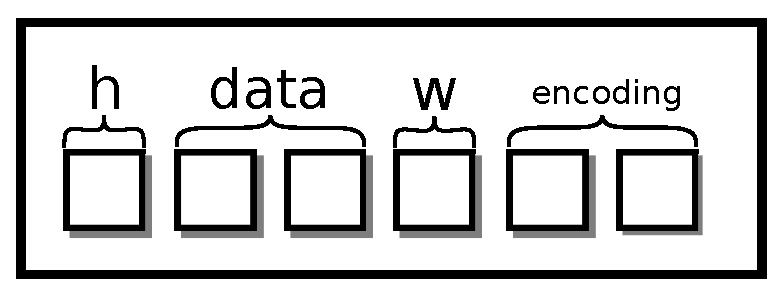
\includegraphics[width=.7\textwidth]{appendix/drawings/struct_clean.eps}
\caption{Six box struct}
\label{fig:clean_struct}
\end{figure}

However, with struct packing, it would conceptually look like this:

\begin{lstlisting}[language=C]
struct picture{
  int height;
  char slop1[4];
  pixel** data;
  int width;
  char slop2[4];
  char* encoding;
}
\end{lstlisting}

Visually, we'd add two extra boxes to our diagram

\begin{figure}[H]
\centering
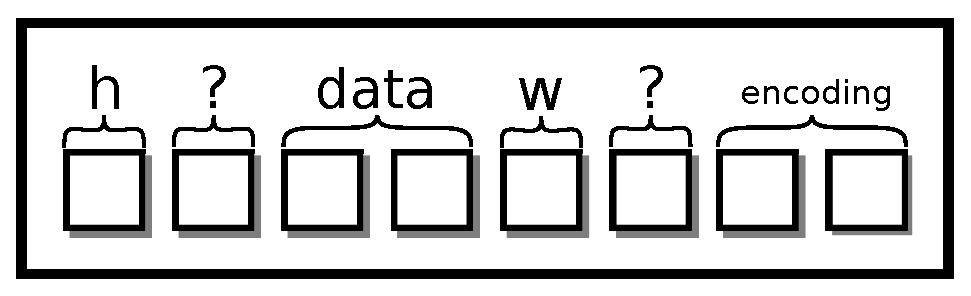
\includegraphics[width=.7\textwidth]{appendix/drawings/struct_slop.eps}
\caption{Eight box struct, two boxes of slop}
\label{fig:sloppy_struct}
\end{figure}

This padding is common on a 64-bit system.
Other time, a processor supports unaligned access, leaving the compiler able to pack structs.
What does this mean?
We can have a variable start at a non-64-bit boundary.
The processor will figure out the rest.
To enable this, set an attribute.

\begin{lstlisting}[language=C]
struct __attribute__((packed, aligned(4))) picture{
  int height;
  pixel** data;
  int width;
  char* encoding;
}
\end{lstlisting}

Now our figure will look like the clean struct as in figure  \ref{fig:clean_struct}
But now, every time the processor needs to access \keyword{data} or \keyword{encoding},
two memory accesses are required.
A possible alternative is to reorder the struct.

\begin{lstlisting}[language=C]
struct picture{
  int height;
  int width;
  pixel** data;
  char* encoding;
}
\end{lstlisting}

\section{Stack Smashing}

Each thread uses a stack memory.
The stack `grows downwards' - if a function calls another function, then the stack is extended to smaller memory addresses.
Stack memory includes non-static automatic (temporary) variables, parameter values, and the return address.
If a buffer is too small some data (e.g.~input values from the user), then there is a real possibility that other stack variables and even the return address will be overwritten.
The precise layout of the stack's contents and order of the automatic variables is architecture and compiler dependent. With a little investigative work, we can learn how to deliberately smash the stack for a particular architecture.

The example below demonstrates how the return address is stored on the stack.
For a particular 32 bit architecture \href{http://cs-education.github.io/sys/}{Live Linux Machine}, we determine that the return address is stored at an address two pointers (8 bytes) above the address of the automatic variable.
The code deliberately changes the stack value so that when the input function returns, rather than continuing on inside the main method, it jumps to the exploit function instead.

\begin{lstlisting}[language=C]
// Overwrites the return address on the following machine:
// http://cs-education.github.io/sys/
#include <stdio.h>
#include <stdlib.h>
#include <unistd.h>

void breakout() {
  puts("Welcome. Have a shell...");
  system("/bin/sh");
}
void input() {
  void *p;
  printf("Address of stack variable: %p\n", &p);
  printf("Something that looks like a return address on stack: %p\n", *((&p)+2));
  // Let's change it to point to the start of our sneaky function.
  *((&p)+2) = breakout;
}
int main() {
  printf("main() code starts at %p\n",main);

  input();
  while (1) {
    puts("Hello");
    sleep(1);
  }

  return 0;
}
\end{lstlisting}

There are \href{https://en.wikipedia.org/wiki/Stack_buffer_overflow}{a lot} of ways that computers tend to get around this.


\section{Compiling and Linking}

This is a high-level overview from the time you compile your program to the time you run your program.
We often know that compiling your program is easy.
You run the program through an IDE or a terminal, and it just works.

\begin{lstlisting}[language=bash]
$ cat main.c
#include <stdio.h>

int main() {
    printf("Hello World!\n");
    return 0;
}
$ gcc main.c -o main
$ ./main
Hello World!
$
\end{lstlisting}

Here are the rough stages of compiling for gcc.

\begin{enumerate}
\item Preprocessing: The preprocessor expands all preprocesor directives.
\item Parsing: The compiler parses the text file for function declarations, variable declarations, etc.
\item Assembly Generation: The compiler then generates assembly code for all the functions after some optimizations if enabled.
\item Assembling: The assembler turns the assembly into 0s and 1s and creates an object file. This object file maps names to pieces of code.
\item Static Linking: The linker then takes a series of objects and static libraries and resolves references of variables and functions from one object file to another. The linker then finds the main method and makes that the entry point for the function. The linker also notices when a function is meant to be dynamically linked. The compiler also creates a section in the executable that tells the operating system that these functions need addresses right before running. 
\item Dynamic Linking: As the program is getting ready to be executed, the operating system looks at what libraries that the program needs and links those functions to the dynamic library.
\item The program is run.
\end{enumerate}

Further classes will teach you about parsing and assembly -- preprocessing is an extension of parsing.
Most classes won't teach you about the two different types of linking though.
Static linking a library is similar to combining object files.
To create a static library, a compiler combines different object files to create one executable.
A static library is literally is an archive of object files.
These libraries are useful when you want your executable to be secure, you know all the code that is being included into your executable, and portable, all the code is bundled with your executable meaning no additional installs.

The other type is a dynamic library.
Typically, dynamic libraries are installed user-wide or system-wide and are accessible by most programs.
Dynamic libraries' functions are filled in right before they are run.
There are a number of benefits to this.

\begin{itemize}
\item Lower code footprint for common libraries like the C standard library
\item Late binding means more generalized code and less reliance on specific behavior.
\item Differentiation means that the shared library can be updated while keeping the executable the same.
\end{itemize}

There are a number of drawbacks as well.

\begin{itemize}
\item All the code is no longer bundled into your program. This means that users have to install something else.
\item There could be security flaws in the other code leading to security exploits in your program.
\item Standard Linux allows you to "replace" dynamic libraries, leading to possible social engineering attacks.
\item This adds additional complexity to your application. Two identical binaries with different shared libraries could lead to different results.
\end{itemize}



\subsubsection{Explanation of the Fork-FILE Problem}

To parse the \href{http://pubs.opengroup.org/onlinepubs/9699919799.2008edition/functions/V2_chap02.html}{POSIX documentation}, we'll have to go deep into the terminology.
The sentence that sets the expectation is the following

\begin{quote}
The result of function calls involving any one handle (the "active handle") is defined elsewhere in this volume of POSIX.1-2008, but if two or more handles are used, and any one of them is a stream, the application shall ensure that their actions are coordinated as described below. If this is not done, the result is undefined.
\end{quote}

What this means is that if we don't follow POSIX to the letter when using two file descriptors that refer to the same description across processes, we get undefined behavior.
To be technical, the file descriptor must have a ``position'' meaning that it needs to have a beginning and an end like a file, not like an arbitrary stream of bytes.
POSIX then goes on to introduce the idea of an active handle, where a handle may be a file descriptor or a \keyword{FILE*} pointer.
File handles don't have a flag called ``active''.
An active file descriptor is one that is currently being used for reading and writing and other operations (such as \keyword{exit}).
The standard says that before a \keyword{fork} that the \textit{application} or your code must execute a series of steps to prepare the state of the file.
In simplified terms, the descriptor needs to be closed, flushed, or read to its entirety -- the gory details are explained later.

\begin{quote}
For a handle to become the active handle, the application shall ensure that the actions below are performed between the last use of the handle (the current active handle) and the first use of the second handle (the future active handle). The second handle then becomes the active handle. All activity by the application affecting the file offset on the first handle shall be suspended until it again becomes the active file handle. (If a stream function has as an underlying function one that affects the file offset, the stream function shall be considered to affect the file offset.)
\end{quote}

Summarizing as if two file descriptors are actively being used, the behavior is undefined.
The other note is that after a fork, the library code must prepare the file descriptor as if the other process were to make the file active at any time.
The last bullet point concerns itself with how a process prepares a file descriptor in our case.

\begin{quote}
If the stream is open with a mode that allows reading and the underlying open file description refers to a device that is capable of seeking, the application shall either perform an fflush(), or the stream shall be closed.
\end{quote}

The documentation says that the child needs to perform an fflush or close the stream because the file descriptor needs to be prepared in case the parent process needs to make it active.
glibc is in a no-win situation if it closes a file descriptor that the parent may expect to be open, so it'll opt for the fflush on exit because exit in POSIX terminology counts as accessing a file.
That means that for our parent process, this clause gets triggered.

\begin{quote}
If any previous active handle has been used by a function that explicitly changed the file offset, except as required above for the first handle, the application shall perform an lseek() or fseek() (as appropriate to the type of handle) to an appropriate location.
\end{quote}

Since the child calls fflush and the parent didn't prepare, the operating system chooses to where the file gets reset.
Different file systems will do different things which are supported by the standard.
The OS may look at modification times and conclude that the file hasn't changed so no resets are needed or may conclude that exit denotes a change and needs to rewind the file back to the beginning.


\section{Banker's Algorithm}

We can start with a single resource Banker's Algorithm.
Consider a banker, who has a finite amount of money.
With a finite amount of money, she wants to make loans and eventually get her money back.
Let's say that we have a set of $n$ people where each of them has a set amount or a limit $a_i$ ($i$ being the $i$th process) that they need to obtain before they can do any work.
The banker keeps track of how much she has given to each person $l_i$. She maintains an amount of money $p$ with her, at all times.
For people to request money, they do the following:
Consider the state of the system $(A=\{a_1, a_2, ...\}, L_t=\{l_{t,1}, l_{t,2}, ...\}, p)$ at time $t$.
A precondition is that we have $p \geq min(A)$, or we have enough money to suit at least one person.
Also, each person will work for a finite period and give back our money.

\begin{itemize}
  \item A person $j$ requests $m$ from me
        \begin{itemize}
          \item if $m \geq p$, they are denied.
          \item if $m + l_j > a_i$ they are denied
          \item Pretend we are in a new state $(A, L_{t+1}=\{.., l_{t+1, j} = l_{t, j} + m, ...\}, p - m)$ where the process is granted the resource.
        \end{itemize}
  \item if now person $j$ is either satisfied ($l_{t+1,j} == a_j$) or $min(a_i - l_{t+1, i}) \leq p$. In other words, we have enough money to suit one other person. If either, consider the transaction safe and give them the money.
\end{itemize}

Why does this work? Well at the start we are in a safe state -- defined by we have enough money to suit at least one person.
Each of these "loans" results in a safe state.
If we have exhausted our reserve, one person is working and will give us money greater than or equal to our previous "loan", thus putting us in a safe state again.
Since we can always make one additional move, the system can never deadlock.
Now, there is no guarantee that the system won't livelock.
If the process we hope to request something never does, no work will be done -- but not due to deadlock.
This analogy expands to higher orders of magnitude but requires that either a process can do its work entirely or there exists a process whose combination of resources can be satisfied, which makes the algorithm a little more tricky (an additional for loop) but nothing too bad.
There are some notable downsides.

\begin{itemize}
  \item The program first needs to know how much of each resource a process needs. A lot of times that is impossible or the process requests the wrong amount because the programmer didn't foresee it.
  \item The system could livelock.
  \item We know in most systems that resources vary, pipes and sockets for example. This could mean that the runtime of the algorithm could be slow for systems with millions of resources.
  \item Also, this can't keep track of the resources that come and go. A process may delete a resource as a side effect or create a resource. The algorithm assumes a static allocation and that each process performs a non-destructive operation.
\end{itemize}


\section{Clean/Dirty Forks (Chandy/Misra Solution)}

There are many more advanced solutions.
One such solution is by Chandy and Misra \cite{Chandy:1984:DPP:1780.1804}.
This is not a true solution to the dining philosophers problem because it has the requirement that philosophers can speak to each other.
It is a solution that ensures fairness for some notion of fairness.
In essence, it defines a series of rounds that a philosopher must eat in a given round before going to the next one.

We won't detail the proof here because it is a little more involved, but feel free to read more.

\section{Actor Model}

The actor model is another form of synchronization that doesn't have to do anything with negotiating locks or waiting.
The idea is simple.
Each actor can either perform work, create more actors, send messages, or respond to messages.
Any time an actor needs something from another actor, it sends a message.
Most importantly, an actor is only responsible for one thing.
If we were implementing a real-world application, we may have an actor that handles the database, one that handles the incoming connections, one that services the connections, etc.
These actors would pass messages to each other like ``there is a new connection'' from the incoming connection actor to the servicing actor.
The servicing actor may send a data request message to the database actor and a data response message comes back.

While this seems like the perfect solution there are drawbacks.
The first is the actual library of communication needs to be synchronized.
If you don't have a framework that does this already -- like the Message Passing Interface or MPI for High-Performance Computing -- then the framework will have to be built and would most likely be as much work to build efficiently compared to direct synchronization.
Also, the messages now encounter additional overhead for serializing and deserializing or at the least.
And a final drawback is that an actor could take an arbitrarily long time to respond to a message, spurring the need for shadow actors who service the same job.

As mentioned, there are frameworks like \href{https://en.wikipedia.org/wiki/Message\_Passing\_Interface}{Message passing interface} that is somewhat based on the actor model and allows distributed systems in high-performance computing to work effectively, but your mileage may vary
If you want to read further on the model, feel free to glance over the Wikipedia page listed below.
\href{https://en.wikipedia.org/wiki/Actor\_model}{Further reading on the actor model}


\section{Includes and conditionals}

The other preprocessor include is the \keyword{\#include} directive and conditionals.
The include directive is explained by example.

\begin{lstlisting}[language=C]
// foo.h
int bar();
\end{lstlisting}

This is our file \keyword{bar.c} unpreprocessed.

\begin{lstlisting}[language=C]
#include "foo.h"
int bar() {
}
\end{lstlisting}

After preprocessing, the compiler sees this

\begin{lstlisting}[language=C]
// foo.c unpreprocessed
int bar();

int bar() {

}
\end{lstlisting}

The other tool is \gls{preprocessor conditionals}.
If a macro is defined or truthy, that branch is taken.

\begin{lstlisting}[language=C]
int main() {
  #ifdef __GNUC__
  return 1;
  #else
  return 0;
  #endif
}
\end{lstlisting}

Using \keyword{gcc} your compiler would preprocess the source to the following.

\begin{lstlisting}[language=C]
int main() {
  return 1;
}
\end{lstlisting}

Using \keyword{clang} your compiler would preprocess to this.

\begin{lstlisting}[language=C]
int main() {
  return 0;
}
\end{lstlisting}


\subsection{Thread Scheduling}

There are a few ways to split up the work.
These are common to the OpenMP framework \cite{silberschatz2005operating}.

\begin{itemize}
\item \keyword{static scheduling} breaks up the problems into fixed-size chunks (predetermined) and have each thread work on each of the chunks.
  This works well when each of the subproblems takes roughly the same time because there is no additional overhead.
  All you need to do is write a loop and give the map function to each sub-array.
\item \keyword{dynamic scheduling} as a new problem becomes available to have a thread serve it.
  This is useful when you don't know how long the scheduling will take
\item \keyword{guided scheduling} This is a mix of the above with a mix of the benefits and tradeoffs.
  You start with static scheduling and move slowly to dynamic if needed
\item \keyword{runtime scheduling} You have absolutely no idea how long the problems are going to take.
  Instead of deciding it yourself, let the program decide what to do!
\end{itemize}

No need to memorize any of the scheduling routines though.
Openmp is a standard that is an alternative to pthreads.
For example, here is how to parallelize a for loop

\begin{lstlisting}[language=C]
#pragma omp parallel for
for (int i = 0; i < n; i++) {
  // Do stuff
}

// Specify the scheduling as follows
// #pragma omp parallel for scheduling(static)
\end{lstlisting}

Static scheduling will divide the problem into fixed-size chunks
Dynamic scheduling will give a job once the loop is over
Guided scheduling is Dynamic with chunks
Runtime is a whole bag of worms.

\section{threads.h}

We have a lot of threading libraries discussed in the extra section.
We have the standard POSIX threads, OpenMP threads, we also have a new C11 threading library that is built into the standard.
This library provides restricted functionality.

Why use restricted functionality?
The key is in the name.
Since this is the C standard library, it has to be implemented in all operating systems that are compliant which are pretty much all of them.
This means there is first-class portability when using threads.

We won't drone on about the functions.
Most of them are renaming of pthread functions anyway.
If you ask why we don't teach these, there are a few reasons

\begin{enumerate}
\item They are pretty new. Even though the standard came out in roughly 2011, POSIX threads have been around forever.
  A lot of their quirks have been ironed out.
\item You lose expressivity.
  This is a concept that we'll talk about in later chapters, but when you make something portable, you lose some expressivity with the host hardware.
  That means that the threads.h library is pretty bare bones.
  It is hard to set CPU affinities.
  Schedule threads together.
  Efficiently look at the internals for performance reasons.
\item A lot of legacy code is already written with POSIX threads in mind.
  Other libraries like OpenMP, CUDA, MPI will either use POSIX processes or POSIX threads with a begrudging port to Windows.
\end{enumerate}

\section{Modern Filesystems}

While the API for most filesystems have stayed the same on POSIX over the years, the actual filesystems themselves provide lots of important aspects.

\begin{itemize}
\item Data Integrity. File systems use journaling and sometimes checksums to ensure that the data written to is valid. Journalling is a simple invention where the file system writes an operation in a journal. If the filesystem crashes before the operation is complete, it can resume the operation when booted up again using the partial journal.
\item Caching. Linux does a good job of caching file system operations like finding inodes. This makes disk operations seem nearly instant. If you want to see a slow system, look at Windows with FAT/NTFS. Disk operations need to be cached by the application, or it will burn through the CPU.
\item Speed. On spinning disk machines, data that is toward the end of a metallic platter will spin faster (angular velocity is farther from the center). Programs used this to reduce time loading large files like movies in a video editing piece of software. SSDs don't have this problem because there is no spinning disk, but they will portion off a section of their space to be used as "swap space" for fiels.
\item Parallelism. Filesystems with multiple heads (for physical hard disks) or multiple controllers (for SSDs) can utilize parallelism by multiplexing the PCIe slot with data, always serving some data to the application whenever possible.
\item Encryption. Data can be encrypted with one or more keys. A good example of this is Apple's APFS file systems.
\item Redundancy. Sometimes data can be replicated to blocks to ensure that the data is always available.
\item Efficient Backups. Many of us have data that we can't store on the cloud for one reason or another. It is useful that when a filesystems is either being used as a backup medium or is the source to the backup that it is able to calculate what has changed efficiently, compress files, and sync between the external drive.
\item Integriy and Bootability. File systems need to be resillient to bit flipping. Most readers have their operating system installed on the same paritition as the file system that they used to do different operations. The file system needs to make sure a stray read or write doesn't destroy the boot sector -- meaning your computer can't start up again.
\item Fragmentation. Just like a memory allocator, allocating space for a file leads to both internal and external fragmentation. The same caching benefit occurs when disk blocks for a single file are located next to each other. File systems need to perform well under low, high, and possible fragmentation usage.
\item Distributed. Sometimes, the filesystem should be single machine fault tolerant. Hadoop and other distributed file system allow you to do that.
\end{itemize}

\subsection{Cutting Edge File systems}

There are a few filesystem hardware nowadays that are truly cutting edge.
The one we'd briefly like to touch on is AMD's StoreMI.
We aren't trying to sell AMD chipsets, but the featureset of StoreMI warrants a mention.

StoreMI is a hardware microcontroller that analyzes how the operating system accesses files and moves files/blocks around to speed up the load time.
A common usage can be imagined as having a fast, but small capacity SSD and a slower, large capcity HDD.
To make it seem like all the files are on an SSD, the StoreMI matches the pattern of file access.
If you are starting up Windows, Windows will often access many files in the same order.
StoreMI takes note of that and when the microcontroller notices it is starting the boot, it will move files from the HDD drive to the SSD before they are requested by the operating system.
By the time the operating system needs then, they are already on the SSD.
StoreMI also does this with other applications as well.
The technology still has a lot to be desired for, but it is an interesting intersection of data and pattern matching with filesystems.


\section{Linux Scheduling}

As of February 2016, Linux by default uses the \emph{Completely Fair Scheduler} for CPU scheduling and the Budget Fair Scheduling ``BFQ'' for I/O scheduling. Appropriate scheduling can have a significant impact on throughput and latency. Latency is important for interactive and soft-real time applications such as audio and video streaming. See the discussion and comparative benchmarks \href{https://lkml.org/lkml/2014/5/27/314}{here} for more information.

Here is how the CFS schedules

\begin{itemize}
\tightlist
\item
  The CPU creates a Red-Black tree with the processes virtual runtime (runtime / nice\_value) and sleeper fairness flag -- if the process is waiting on something, give it the CPU when it is done waiting.
\item
  Nice values are the kernel's way of giving priority to certain processes, the lower nice value the higher priority.
\item
  The kernel chooses the lowest one based on this metric and schedules that process to run next, taking it off the queue. Since the red-black tree is self-balancing this operation is guaranteed \(O(log(n))\) (selecting the min process is the same runtime)
\end{itemize}

Although it is called the Fair Scheduler there are a fair bit of problems.

\begin{itemize}
\tightlist
\item
  Groups of processes that are scheduled may have imbalanced loads so the scheduler roughly distributes the load. When another CPU gets free it can only look at the average load of a group schedule, not the individual cores. So the free CPU may not take the work from a CPU that is burning so long as the average is fine.
\item
  If a group of processes is running on non-adjacent cores then there is a bug. If the two cores are more than a hop away, the load balancing algorithm won't even consider that core. Meaning if a CPU is free and a CPU that is doing more work is more than a hop away, it won't take the work (may have been patched).
\item
  After a thread goes to sleep on a subset of cores, when it wakes up it can only be scheduled on the cores that it was sleeping on. If those cores are now busy, the thread will have to wait on them, wasting opportunities to use other idle cores.
\item
  To read more on the problems of the Fair Scheduler, read \href{https://blog.acolyer.org/2016/04/26/the-linux-scheduler-a-decade-of-wasted-cores}{here}.
\end{itemize}


\subsection{Implementing Software Mutex}

Yes
With a bit of searching, it is possible to find it in production for specific simple mobile processors today.
Peterson's algorithm is used to implement low-level Linux Kernel locks for the Tegra mobile processor (a system-on-chip ARM process and GPU core by Nvidia) \href{https://android.googlesource.com/kernel/tegra.git/+/android-tegra-3.10/arch/arm/mach-tegra/sleep.S\#58}{Link to Lock Source}

In general now, CPUs and C compilers can re-order CPU instructions or use CPU-core-specific local cache values that are stale if another core updates the shared variables.
Thus a simple pseudo-code to C implementation is too naive for most platforms.
Warning, here be dragons!
Consider this advanced and gnarly topic but (spoiler alert) a happy ending.
Consider the following code,

\begin{lstlisting}[language=C]
while(flag2) { /* busy loop - go around again */
\end{lstlisting}

An efficient compiler would infer that \keyword{flag2} variable is never changed inside the loop, so that test can be optimized to \keyword{while(true)} Using \keyword{volatile} goes some way to prevent compiler optimizations of this kind.

Let's say that we solved this by telling the compiler not to optimize.
Independent instructions can be re-ordered by an optimizing compiler or at runtime by an out-of-order execution optimization by the CPU.

A related challenge is that CPU cores include a data cache to store recently read or modified main memory values.
Modified values may not be written back to main memory or re-read from memory immediately.
Thus data changes, such as the state of a flag and turn variable in the above example, may not be shared between two CPU codes.

But there is a happy ending.
Modern hardware addresses these issues using `memory fences' also known as a memory barrier.
This prevents instructions from getting ordered before or after the barrier.
There is a performance loss, but it is needed for correct programs!

Also, there are CPU instructions to ensure that main memory and the CPU's cache is in a reasonable and coherent state.
Higher-level synchronization primitives, such as \keyword{pthread\_mutex\_lock} are will call these CPU instructions as part of their implementation.
Thus, in practice, surrounding critical sections with a mutex lock and unlock calls is sufficient to ignore these lower-level problems.

For further reading, we suggest the following web post that discusses implementing Peterson's algorithm on an x86 process and the Linux documentation on memory barriers.
\begin{enumerate}
\item \href{http://bartoszmilewski.com/2008/11/05/who-ordered-memory-fences-on-an-x86/}{Memory Fences}
\item \href{http://lxr.free-electrons.com/source/Documentation/memory-barriers.txt}{Memory Barriers}
\end{enumerate}


\section{The Curious Case of Spurious Wakeups}

Condition variables need a mutex for a few reasons.
One is simply that a mutex is needed to synchronize the changes of the \textit{condition variable} across threads.
Imagine a condition variable needing to provide its own internal synchronization to ensure its data structures work correctly.
Often, we use a mutex to synchronize other parts of our code, so why double the cost of using a condition variable.
Another example relates to high priority systems.
Let's examine a code snippet.

\begin{lstlisting}[language=C]
// Thread 1
while (answer < 42) pthread_cond_wait(cv);

// Thread 2
answer = 42
pthread_cond_signal(cv);
\end{lstlisting}

\\
\begin{center}
\begin{table}[h]
\caption{Signaling without Mutex}
\begin{tabular}{|c|c|}
  Thread 1 & Thread 2 \\ \hline
  while(answer < 42) & \\
  & answer++ \\
  & pthread\_cond\_signal(cv) \\
  pthread\_cond\_wait(cv)
\end{tabular}
\end{table}
\end{center}
\\
The problem here is that a programmer expects the signal to wake up the waiting thread.
Since instructions are allowed to be interleaved without a mutex, this causes an interleaving that is confusing to application designers.
Note that technically the API of the condition variable is satisfied.
The wait call \textit{happens-after} the call to signal, and signal is only required to release at most a single thread whose call to wait \textit{happened-before}.

Another problem is the need to satisfy real-time scheduling concerns which we only outline here.
In a time-critical application, the waiting thread with the \emph{highest priority} should be allowed to continue first.
To satisfy this requirement the mutex must also be locked before calling \keyword{pthread\_cond\_signal} or \keyword{pthread\_cond\_broadcast}.
For the curious, \href{https://groups.google.com/forum/?hl=ky\#!msg/comp.programming.threads/wEUgPq541v8/ZByyyS8acqMJ}{here is a longer, historical discussion}.

\section{Condition Wait Example}

The call \keyword{pthread\_cond\_wait} performs three actions:

\begin{enumerate}
\item Unlock the mutex. The mutex must be locked.
\item Sleeps until \keyword{pthread\_cond\_signal} is called on the same condition variable.
\item Before returning, locks the mutex.
\end{enumerate}

Condition variables are \emph{always} used with a mutex lock.
Before calling \emph{wait}, the mutex lock must be locked and \emph{wait} must be wrapped with a loop.

\begin{lstlisting}[language=C]
pthread_cond_t cv;
pthread_mutex_t m;
int count;

// Initialize
pthread_cond_init(&cv, NULL);
pthread_mutex_init(&m, NULL);
count = 0;

// Thread 1
pthread_mutex_lock(&m);
while (count < 10) {
  pthread_cond_wait(&cv, &m);
  /* Remember that cond_wait unlocks the mutex before blocking (waiting)! */
  /* After unlocking, other threads can claim the mutex. */
  /* When this thread is later woken it will */
  /* re-lock the mutex before returning */
}
pthread_mutex_unlock(&m);

//later clean up with pthread_cond_destroy(&cv); and mutex_destroy


// Thread 2:
while (1) {
  pthread_mutex_lock(&m);
  count++;
  pthread_cond_signal(&cv);
  /* Even though the other thread is woken up it cannot not return */
  /* from pthread_cond_wait until we have unlocked the mutex. This is */
  /* a good thing! In fact, it is usually the best practice to call */
  /* cond_signal or cond_broadcast before unlocking the mutex */
  pthread_mutex_unlock(&m);
}
\end{lstlisting}

This is a pretty naive example, but it shows that we can tell threads to wake up in a standardized manner.
In the next section, we will use these to implement efficient blocking data structures.


\section{Implementing CVs with Mutexes Alone}

Implementing a condition variable using only a mutex isn't trivial.
Here is a sketch of how we could do it.

\begin{lstlisting}[language=C]
typedef struct cv_node_ {
  pthread_mutex_t *dynamic;
  int is_awoken;
  struct cv_node_ *next;
} cv_node;

typedef struct {
  cv_node_ *head
} cond_t

void cond_init(cond_t *cv) {
  cv->head = NULL;
  cv->dynamic = NULL;
}

void cond_destroy(cond_t *cv) {
  // Nothing to see here
  // Though may be useful for the future to put pieces
}

static int remove_from_list(cond_t *cv, cv_node *ptr) {
  // Function assumes mutex is locked
  // Some sanity checking
  if (ptr == NULL) {
    return
  }

  // Special case head
  if (ptr == cv->head) {
    cv->head = cv->head->next;
    return;
  }

  // Otherwise find the node previous
  for (cv_node *prev = cv->head; prev->next; prev = prev->next) {
    // If we've found it, patch it through
    if (prev->next == ptr) {
      prev->next = prev->next->next;
      return;
    }
    // Otherwise keep walking
    prev = prev->next;
  }

  // We couldn't find the node, invalid call

}
\end{lstlisting}

This is all the boring definitional stuff.
The interesting stuff is below.

\begin{lstlisting}[language=C]
void cond_wait(cond_t *cv, pthread_mutex_t *m) {
  // See note (dynamic) below
  if (cv->dynamic == NULL) {
    cv->dynamic = m
  } else if (cv->dynamic != m) {
    // Error can't wait with a different mutex!
    abort();
  }
  // mutex is locked so we have the critical section right now
  // Create linked list node _on the stack_
  cv_node my_node;
  my_node.is_awoken = 0;
  my_node.next = cv->head;
  cv->head = my_node.next;
  pthread_mutex_unlock(m);

  // May do some cache busting here
  while(my_node == 0) {
    pthread_yield();
  }

  pthread_mutex_lock(m);
  remove_from_list(cv, &my_node);

  // The dynamic binding is over
  if (cv->head == NULL) {
    cv->dynamic = NULL;
  }
}

void cond_signal(cond_t *cv) {
  for (cv_node *iter = cv->head; iter; iter = iter->next) {
    // Signal makes sure one thread that has not woken up
    // is woken up
    if (iter->is_awoken == 0) {
      // DON'T remove from the linked list here
      // There is no mutual exclusion, so we could
      // have a race condition
      iter->is_awoken = 1;
      return;
    }
  }

  // No more threads to free! No-op
}

void cond_broadcast(cond_t *cv) {
  for (cv_node *iter = cv->head; iter; iter = iter->next) {
    // Wake everyone up!
    iter->is_awoken = 1;
  }
}
\end{lstlisting}

So how does this work?
Instead of allocating space which could lead to deadlock.
We keep the data structures or the linked list nodes on each thread's stack.
The linked list in the wait function is created \textbf{While the thread has the mutex lock} this is important because we may have a race condition on the insert and removal.
A more robust implementation would have a mutex per condition variable.

What is the note about (dynamic)?
In the pthread man pages, wait creates a runtime binding to a mutex. This means that after the first call is called, a mutex is associated with a condition variable while there is still a thread waiting on that condition variable.
Each new thread coming in must have the same mutex, and it must be locked.
Hence, the beginning and end of wait (everything besides the while loop) are mutually exclusive.
After the last thread leaves, meaning when head is NULL, then the binding is lost.

The signal and broadcast functions merely tell either one thread or all threads respectively that they should be woken up.
\textbf{It doesn't modify the linked lists because there is no mutex to prevent corruption if two threads call signal or broadcast}

Now an advanced point.
Do you see how a broadcast could cause a spurious wakeup in this case? Consider this series of events.

\begin{enumerate}
\item Some number more than 2 threads start waiting
\item Another thread calls broadcast.
\item That thread calling broadcast is stopped before it wake any threads.
\item Another thread calls wait on the condition variable and adds itself to the queue.
\item Broadcast iterates through and frees all of the threads.
\end{enumerate}

There is no assurance as to \textit{when} the broadcast was called and when threads were added in a high-performance mutex.
The ways to prevent this behavior are to include Lamport timestamps or require that broadcast be called with the mutex in question.
That way something that \textit{happens-before} the broadcast call doesn't get signaled after.
The same argument is put forward for signal too.

Did you also notice something else?
\textbf{This is why we ask you to signal or broadcast before you unlock}.
If you broadcast after you unlock, the time that broadcast takes could be infinite!
\begin{enumerate}
\item Broadcast is called on a waiting queue of threads
\item First thread is freed, broadcast thread is frozen. Since the mutex is unlocked, it locks and continues.
\item It continues for such a long time that it calls broadcast again.
\item With our implementation of a condition variable, this would be terminated.
  If you had an implementation that appended to the tail of the list and iterated form the head to the tail, this could go on infinitely many times.
\end{enumerate}

In high-performance systems, we want to make sure that each thread that calls wait isn't passed by another thread that calls wait.
With the current API that we have, we can't assure that.
We'd have to ask users to pass in a mutex or use a global mutex.
Instead, we tell programmers to always signal or broadcast before unlocking.


\section{Higher Order Models of Synchronization}

When using atomics, you need to specify the right model of synchronization to ensure a program behaves correctly.
You can read more about them \href{https://gcc.gnu.org/wiki/Atomic/GCCMM/AtomicSync}{On the gcc wiki}
These examples are adapted from those.

\subsection{Sequentially Consistent}

Sequentially consistent is the simplest, least error-prone and most expensive model. This model says that any change that happens, all changes before it will be synchronized between all threads.

\begin{verbatim}
    Thread 1                    Thread 2
    1.0 atomic_store(x, 1)
    1.1 y = 10                  2.1 if (atomic_load(x) == 0)
    1.2 atomic_store(x, 0);     2.2    y != 10 && abort();
\end{verbatim}

Will never quit.
This is because either the store happens before the if statement in thread 2 and y == 1 or the store happens after and x does not equal 2.

\subsection{Relaxed}

Relaxed is a simple memory order providing for more optimizations.
This means that only a particular operation needs to be atomic.
One can have stale reads and writes, but after reading the new value, it won't become old.

\begin{verbatim}
    -Thread 1-              -Thread 2-
    atomic_store(x, 1);     printf("%d\n", x) // 1
    atomic_store(x, 0);     printf("%d\n", x) // could be 1 or 0
                            printf("%d\n", x) // could be 1 or 0
\end{verbatim}

But that means that previous loads and stores don't need to affect other threads.
In the previous example, the code can now fail.

\subsection{Acquire/Release}

The order of atomic variables don't need to be consistent -- meaning if atomic var y is assigned to 10 then atomic var x to be 0 those don't need to propagate, and a threa could get stale reads.
Non-atomic variables have to get updated in all threads though.

\subsection{Consume}

Imagine the same as above except non-atomic variables don't need to get updated in all threads.
This model was introduced so that there can be an Acquire/Release/Consume model without mixing in Relaxed because Consume is similar to relax.

\section{Actor Model and Goroutines}

There are a \textit{lot} of other methods of concurrency than described in this book.
Posix threads are the finest grained thread construct, allowing for tight control of the threads and the CPU.
Other languages have their abstractions.
We'll talk about a language go that is similar to C in terms of simplicity and design, go or golang
To get the 5 minute introduction, feel free to read \href{https://learnxinyminutes.com/docs/go/}{the learn x in y guide} for go.
Here is how we create a "thread" in go.

\begin{lstlisting}[language=golang]
func hello(out) {
    fmt.Println(out);
}

func main() {
    to_print := "Hello World!"
    go hello(to_print)
}
\end{lstlisting}

This actually creates what is known as a goroutine.
A goroutine can be thought of as a lightweight thread.
Internally, it is a worker pool of threads that executes instructions of all the running goroutines.
When a goroutine needs to be stopped, it is frozen and "context switched" to another thread.
Context switch is in quotes because this is done at the run time level versus real context switching which is done at the operating system level.

The advantage to gofuncs is pretty self explanatory.
There is no boilerplate code, or joining, or odd casting \keyword{void *}.

We can still use mutexes in go to perform our end result.
Consider the counting example as before.

\begin{lstlisting}[language=golang]
var counter = 0;
var mut sync.Mutex;
var wg sync.WaitGroup;
 
func plus() {
  mut.Lock()
  counter += 1
  mut.Unlock()
  wg.Done()
}

func main() {
  num := 10
  wg.Add(num);
  for i := 0; i < num; i++ {
    go plus()
  }

  wg.Wait()

  fmt.Printf("%d\n", counter);

}
\end{lstlisting}

But that's boring and error prone.
Instead, let's use the actor model.
Let's designate two actors.
One is the main actor that will be performing the main instruction set.
The other actor will be the counter.
The counter is responsible for adding numbers to an internal variable.
We'll send messages between the threads when we want to add and see the value.


\begin{lstlisting}[language=golang]
const (
  addRequest = iota;
  outputRequest = iota;
)

func counterActor(requestChannel chan int, outputChannel chan int) {
  counter := 0

  for {
    req := <- requestChannel;
    if req == addRequest {
      counter += 1
    } else if req == outputRequest {
      outputChannel <- counter
    }
  }
}

func main() {
  // Set up the actor
  requestChannel := make(chan int)
  outputChannel := make(chan int)
  go counterActor(requestChannel, outputChannel)

  num := 10
  for i := 0; i < num; i++ {
    requestChannel <- addRequest
  }
  requestChannel <- outputRequest
  new_count := <- outputChannel
  fmt.Printf("%d\n", new_count);
}
\end{lstlisting}

Although there is a bit more boilerplate code, we don't have mutexes anymore!
If we wanted to scale this operation and do other things like increment by a number, or write to a file, we can have that particular actor take care of it.
This differentiation of responsibilities is important to make sure your design scales well.
There are even libraries that handle all of the boilerplate code as well.

\section{Scheduling Conceptually}

\textbf{This section could be useful for those that like to analyze these algorithms mathematically}

If your co-worker asked you what scheduling algorithm to use, you may not have the tools to analyze each algorithm.
So, let's think about scheduling algorithms at a high level and break them down by their times.
We will be evaluating this in the context of a random process timing, meaning that each process takes a random but finite amount of time to finish.

Just a refresher, here are the terms.

\begin{center}
\begin{table}[h]
\caption{Scheduling Variables}
\begin{tabular}{|c|c|}
  Concept & Meaning \\ \hline
  Start time & The time the scheduler first started work \\
  End time & When the scheduler finished the process \\
  Arrival time & When the job first arrived at the scheduler \\
  Run time & How long does the process take to run if there is no preemption
\end{tabular}
\end{table}
\end{center}

And here are the measures we are trying to optimize.

\begin{center}
\begin{table}[h]
\caption{Scheduling Measures of Efficiency}
\begin{tabular}{|c|c|}
  Measure & Formula \\ \hline
  Response Time & Start time minus Arrival time\\
  Turnaround time & End time minus Arrival time\\
  Wait time & End time minus Arrival time minus Run time \\
\end{tabular}
\end{table}
\end{center}

Different use cases will be discussed after.
Let the maximum amount of time that a process run be equal to $S$.
We will also assume that there are a finite number of processes running at any given time $c$.
Here are some concepts from queueing theory that you'll need to know that will help simplify the theories.

\begin{enumerate}
\item Queueing theory involves a random variable controlling the interarrival time -- or the time between two different processes arriving.
  We won't name this random variable, but we will assume that (1) it has a mean of $\lambda$ and (2) it is distributed as a Poisson random variable.
  This means the probability of getting a process $t$ units after getting another process is $\lambda^t * \frac{\exp(-\lambda)}{t!}$ where $t!$ can be approximated by the gamma function when dealing with real values.
\item We will be denoting the service time $S$, and deriving the waiting time $W$, and the response time $R$; more specifically the expected values of all of those variables $E[S]$ deriving turnaround time is simply $S + W$.
  For clarity, we will introduce another variable $N$ that is the number of people currently in the queue.
  A famous result in queueing theory is Little's Law which states $E[N] = \lambda E[W]$ meaning that the number of people waiting is the arrival rate times the expected waiting time (assuming the queue is in a steady state).
\item We won't make many assumptions about how much time it takes to run each process except that it will take a finite amount of time -- otherwise this gets almost impossible to evaluate.
We will denote two variables that $\frac{1}{\mu}$ is the mean of the waiting time and that the coefficient of variation $C$ is defined as $C^2 = \frac{var(S)}{E[S]^2}$ to help us control for processes that take a while to finish.
An important note is that when $C > 1$ we say that the running times of the process are variadic. We will note below that this rockets up the wait and response times for FCFS quadratically.
\item $\rho = \frac{\lambda}{\mu} < 1$ Otherwise, our queue would become infinitely long
\item We will assume that there is one processor. This is known as an M/G/1 queue in queueing theory.
\item We'll leave the service time as an expectation $S$ otherwise we may run into over-simplifications with the algebra.
  Plus it is easier to compare different queueing disciplines with a common factor of service time.
\end{enumerate}

\subsection{First Come First Served}

All results are from Jorma Virtamo's lectures on the matter \cite{virtamo}.

\begin{enumerate}
\item The first is expected waiting time.
  \[
  E[W] = \frac{(1 + C^2)}{2}\frac{\rho}{(1 - \rho)} * E[S]
  \]

  What does this say? When given as $\rho \rightarrow 1$ or the mean job arrival rate equals the mean job processing rate, then the wait times get long.
  Also, as the variance of the job increases, the wait times go up.

\item Next is the expected response time

  \[
  E[R] = E[N] * E[S] = \lambda * E[W] * E[S]
  \]
  The response time is simple to calculate, it is the expected number of people ahead of the process in the queue times the expected time to service each of those processes.
  From Little's Law above, we can substitute that for this. Since we already know the value of the waiting time, we can reason about the response time as well.
\item A discussion of the results is shows something cool discovered by Conway and Al \cite{conway1967theory}.
  Any scheduling discipline that isn't preemptive and doesn't take into account the run time of the process or a priority will have the same wait, response, and turnaround time.
  We will often use this as a baseline.
\end{enumerate}

\subsection{Round Robin or Processor Sharing}

It is hard to analyze Round Robin from a probabilistic sense because it is so state based.
The next job that the scheduler schedules requires it to remember the previous jobs.
Queueing theory developers have made an assumption that the time quanta is roughly zero -- ignoring context switching and the like.
This leads way into processor sharing.
Many different tasks can get worked on at the same time but experience a slowdown.
All of these proofs will be adapted from Harchol-Balter's book \cite{harchol2013performance}.
We highly recommend checking out the books if you are interested.
The proofs are intuitive for people who don't have a background in queueing theory.

\begin{enumerate}
  \item Before we jump to the answer let's reason about this.
    With our new-found abstraction, we essentially have an FCFS queue where we are going to be working on each job a little slower than before.
    Since we are always working on a job

    \[
    E[W] = 0
    \]

  Under a non-strict analysis of processor sharing though, the number of time that the scheduler waits is best approximated by the number of times the scheduler need to wait.
  You'll need $\frac{E[S]}{Q}$ service periods where $Q$ is the quanta, and you'll need about $E[N] * Q$ time in between those periods.
  Leading to an average time of
  \[
  E[W] = E[S] * E[N]
  \]

  The reason this proof is non-rigorous is that we can't assume that there will always be $E[N] * Q$ time on average in between cycles because it depends on the state of the system.
  This means we need to factor in various variations in processing delay.
  We also can't use Little's Law in this case because there is no real steady state of the system.
  Otherwise, we'd be able to prove some weird things.

  Interestingly, we don't have to worry about the convoy effect or any new processes coming in.
  The total wait time remains bounded by the number of people in the queue.
  For those of you familiar with tail inequalities since processes arrive according to a Poisson distribution, the probability that we'll get many processes drops off exponentially due to Chernoff bounds (all arrivals are independent of other arrivals).
  Meaning roughly we can assume low variance on the number of processes.
  As long as the service time is reasonable on average, the wait time will be too.

\item The expected response time is
  \[
  E[R] = 0
  \]

  Under strict processor sharing, it is 0 because all jobs are worked on.
  In practice, the response time is.
  \[
  E[R] = E[N] * Q
  \]

  Where $Q$ is the quanta.
  Using Little's Law again, we can find out that
  \[
  E[R] = \lambda E[W] * Q
  \]
\item A different variable is the amount of service time let the service time for processor sharing be defined as $S_{PS}$.
  The slowdown is $E[S_{PS}] = \frac{E[S]}{1 - \rho}$
  Which means as the mean arrival rate equals the mean processing time, then the jobs will take asymptotically as long to finish.
  In the non-strict analysis of processor sharing, we assume that
  \[
    E[S_{RR}] = E[S] + Q * \epsilon, \epsilon > 0
  \]
    $\epsilon$ is the amount of time a context switch takes.

\item That naturally leads to the comparison, what is better?
  The response time is roughly the same comparing the non-strict versions, the wait time is roughly the same, but notice that nothing about the variation of the jobs is put in.
  That's because RR doesn't have to deal with the convoy effect and any variances associated, otherwise FCFS is faster in a strict sense.
  It also takes more time for the jobs to finish, but the overall turnaround time is lower under high variance loads.
\end{enumerate}

\subsection{Non Preemptive Priority}

We will introduce the notation that there are $k$ different priorities and $\rho_i > 0$ is the average load contribution for priority $i$ We are constrained by $\sum\limits_{i=0}^k \rho_i = \rho$.
We will also denote $\rho(x) = \sum\limits_{i=0}^x \rho_i$ which is the load contribution for all higher and similar priority processes to $x$.
The last bit of notation is that we will assume that the probability of getting a process of priority $i$ is $p_i$ and naturally $\sum\limits_{j=0}^k p_j = 1$
 
\begin{enumerate}
\item If $E[W_i]$ is the wait time for priority $i$,
  \[
  E[W_x] = \frac{(1 + C)}{2}\frac{\rho}{(1 - \rho(x))*( 1 - \rho(x-1))} * E[S_i]
  \]
    The full derivation is as always in the book.
    A more useful inequality is that.

    \[
    E[W_x] \leq \frac{1 + C}{2}* \frac{\rho}{(1 - \rho(x))^2} * E[S_i]
    \]
    because the addition of $\rho_x$ can only increase the sum, decrease the denominator or increase the overall function.
  This means that if one is priority 0, then a process only need to wait for the other P0 processes which there should be $\rho C/ (1 - \rho_0)$ P0 processes arrived before to process in FCFS order.
  Then the next priority has to wait for all the others and so on and so forth.

  The expected overall wait time is now

  \[
      E[W] = \sum\limits_{i=0}^k E[W_i] * p_i
  \]

  Now that we have notational soup, let's factor out the important terms.

  \[
      \sum\limits_{i=0}^k \frac{p_i}{(1-\rho(i))^2}
  \]

  Which we compare with FCFS' model of

  \[
      \frac{1}{1-\rho}
  \]

  In words -- you can work this out with experimenting distributions -- if the system has a lot of low priority processes who don't contribute a lot to the average load, your average wait time becomes much lower.

\item The average per process response time is

  \[
  E[R_i] = \sum\limits_{j = 0}^i E[N_j] * E[S_j]
  \]

  Which says that the scheduler needs to wait for all jobs with a higher priority and the same to go before a process can go.
  Imagine a series of FCFS queues that a process needs to wait your turn.
  Using Little's Law for different colored jobs and the formula above we can simplify this

  \[
      E[R_i] = \sum\limits_{j=0}^i \lambda_j E[W_j] * E[S_j]
  \]

  And we can find the average response time by looking at the distribution of jobs

  \[
      E[R] = \sum\limits_{i=0}^k p_i [\sum\limits_{j=0}^k \lambda_j E[W_j] * E[S_j] ]
  \]

  Meaning that we are tied to wait times and service times of all other processes.
  If we break down this equation, we see again if we have a lot of high priority jobs that don't contribute a lot to the load then our entire sum goes down.
  We won't make too many assumptions about the service time for a job because that would interfere with our analysis from FCFS where we left it as an expression.

  \item As for a comparison with FCFS in the average case, it usually does better assuming that we have a smooth probability distribution -- i.e. the probability of getting any particular priority is zero.
  In all of our formulas, we still have some probability mass to put on lower priority processes, bringing the expectation down.
  This statement doesn't hold for all smooth distributions but for most real-world smoothed distributions (which tend to be smooth) they do.

\item This isn't even to mention the idea of utility.
  Utility means that if we gain an amount of happiness by having certain jobs finish, priority and preemptive priority maximize that while balancing out other measures of efficiency.
\end{enumerate}


\subsection{Shortest Job First}
This is a wonderful reduction to priority.
Instead of having discrete priorities, we'll introduce a process that takes $S_t$ time to get serviced.
$T$ is the maximum amount of time a process can run for, our processes cannot run infinitely long.
That means the following definitions hold, overriding the previous definitions in priority

\begin{enumerate}
\item Let
  \[
  \rho(x) = \int_0^x \rho_u du
  \]
  Be the average load contribution up to this point.
\item
  \[
  \int_0^k p_u du = 1
  \] Probability constraint.
\item Etc, replace all the summations above with integrals
\item The only notational difference is we don't have to make any assumptions about the service times of the jobs because they are denoted by service times subscript, all other analyses are the same.
  \item This means if you want low wait times on average compared to FCFS, your distribution needs to be right-skewed.
\end{enumerate}

\subsection{Preemptive Priority}

We will describe priority and SJF's preemptive version in the same section because it is essentially the same as we've shown above.
We'll use the same notation as before.
We will also introduce an additional term $C_i$ which denotes the variation among a particular class

\[
    C_i = \frac{var(S_i)}{E[S_i]}
\]

\begin{enumerate}
\item Response Time. Just a head's up, this isn't going to be pretty.
  \[
  E[R_i] = \frac{\sum\limits_{j=0}^i\frac{(1 + C_j)}{2}}{(1 - \rho(x))*( 1 - \rho(x-1))} * E[S_i]
  \]

  If this looks familiar it should.
  This is the average wait time in the nonpreemptive case with a small change. Instead of using the variance of the entire distribution, we are looking at the variance of each job coming in.
  The whole response times are

  \[
     E[R] = \sum\limits_{i = 0}^k p_i * E[R_i]
  \]

  If lower priorities jobs come in at a higher service time variance, that means our average response times could go down, unless they make up most of the jobs that come in.
  Think of the extreme cases.
  If 99\% of the jobs are high priority and the rest make up the other percent, then the other jobs will get frequently interrupted, but high priority jobs will make up most of the jobs, so the expectation is still low.
  The other extreme is if one percent of jobs are high priority and they come in a low variance.
  That means the chances the system getting a high priority jobs that will take a long time is low, thus making our response times lower on average.
  We only run into trouble if high priority jobs make up a non-negligible amount, and they have a high variance in service times.
  This brings down response times as well as wait times.

\item Waiting Time
  \[
  E[W_i] = E[R_i] + \frac{E[S_i]}{1 - \rho(i)}
  \]

  Taking the expectation among all processes we get

  \[
  E[W] = \sum\limits_{i = 0}^k p_i (E[R_i] + \frac{E[S_i]}{1 - \rho(i)})
  \]

  We can simplify to

  \[
  E[W] = E[R] + \sum\limits_{i=0}^k \frac{E[S_i]p_i}{(1 - \rho(i))}
  \]

  We incur the same cost on response time and then we have to suffer an additional cost based on what the probabilities are of lower priority jobs coming in and taking this job out.
  That is what we call the average interruption time.
  This follows the same laws as before.
  Since we have a variadic, pyramid summation if we have a lot of jobs with small service times then the wait time goes down for both additive pieces.
  It can be analytically shown that this is better given certain probability distributions.
  For example, try with the uniform versus FCFS or the non preemptive version.
  What happens?
  As always the proof is left to the reader.

\item Turnaround Time is the same formula $E[T] = E[S] + E[W]$. This means that given a distribution of jobs that has either low waiting time as described above, we will get low turnaround time -- we can't control the distribution of service times.
\end{enumerate}

\subsection{Preemptive Shortest Job First}

Unfortunately, we can't use the same trick as before because an infinitesimal point doesn't have a controlled variance.
Imagine the comparisons though as the same as the previous section.

\section{Networking Extra}


\subsection{In-depth IPv4 Specification}

The Internet Protocol deals with routing, fragmentation, and reassembly of fragments.
Datagrams are formatted as such

\begin{figure}[H]
  \centering
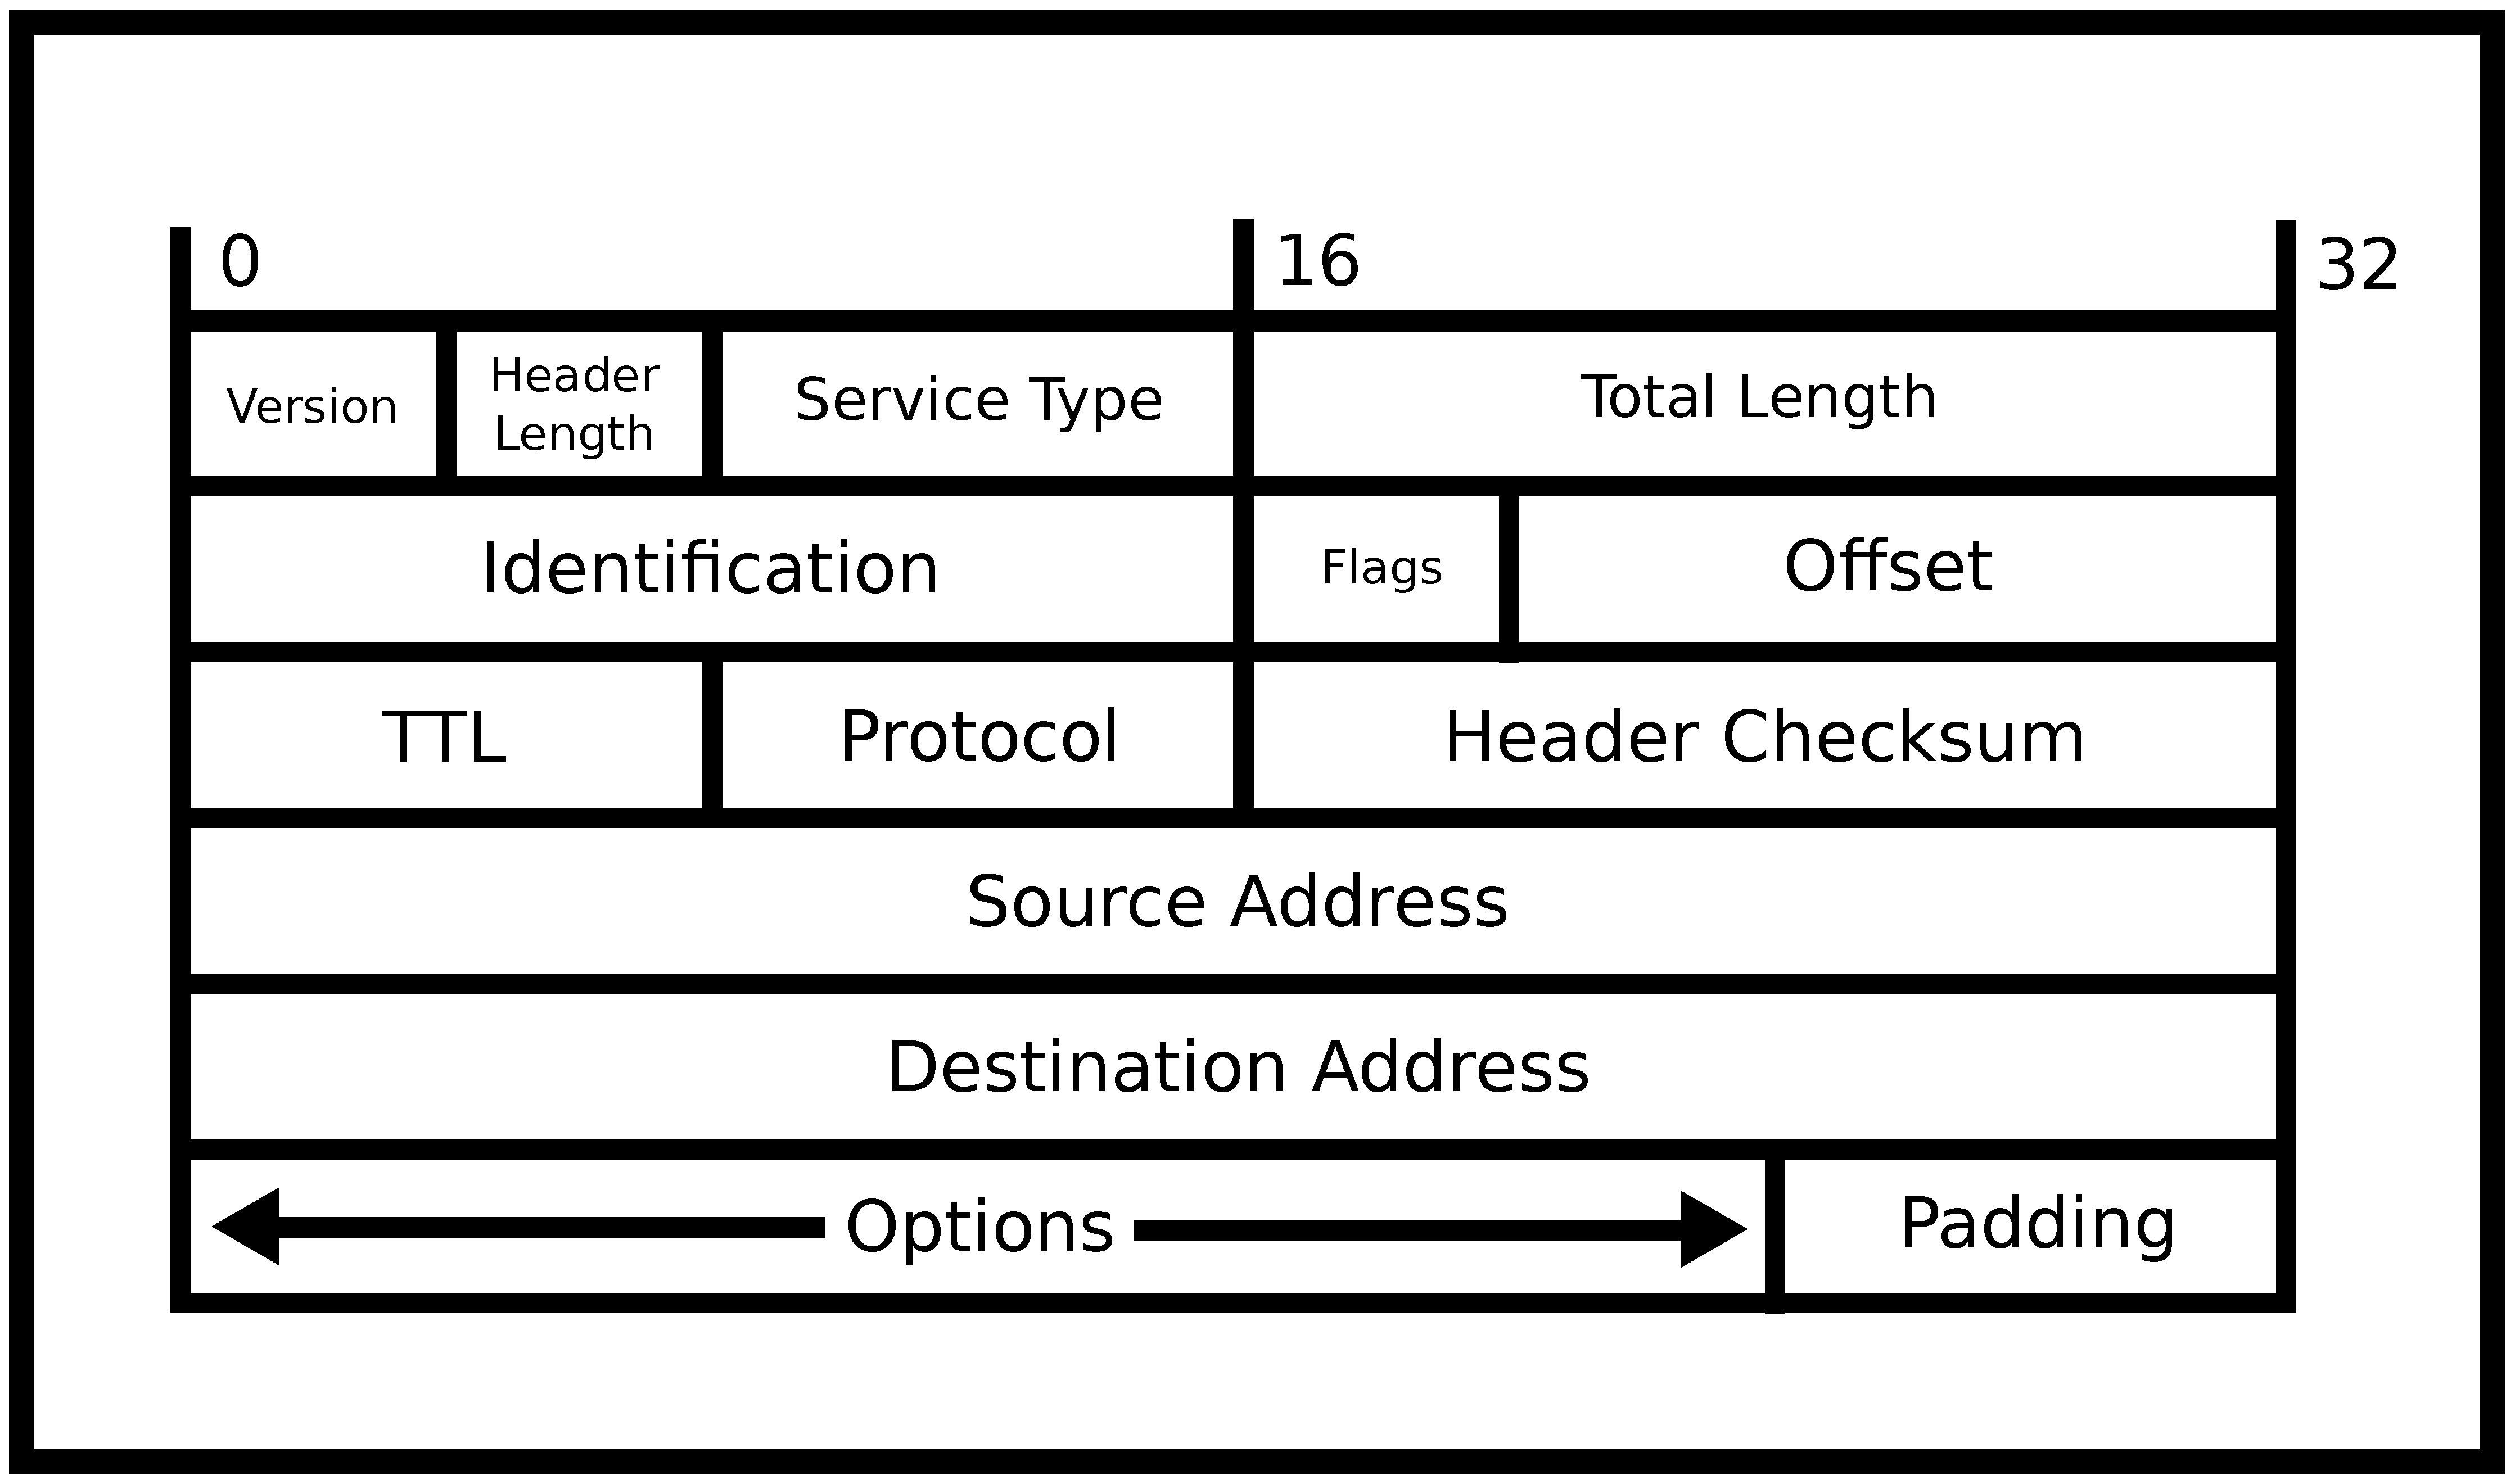
\includegraphics[width=.8\textwidth]{appendix/drawings/ip_datagram.eps}
\caption{IP Datagram divisibility}
\end{figure}

\begin{enumerate}
  \item The first octet is the version number, either 4 or 6
  \item The next octet is how long the header is.
    Although it may seem that the header is a constant size, you can include optional parameters to augment the path that is taken or other instructions.
  \item The next two octets specify the total length of the datagram.
    This means this is the header, the data, the footer, and the padding.
    This is given in multiple of octets, meaning that a value of 20 means 20 octets.
  \item The next two are Identification number.
    IP handles taking packets that are too big to be sent over the physical wire and chunks them up.
    As such, this number identifies what datagram this originally belonged to.
  \item The next octet is various bit flags that can be set.
  \item The next octet and half is fragment number.
    If this packet was fragmented, this is the number this fragment represents
  \item The next octet is time to live.
    So this is the number of "hops" (travels over a wire) a packet is allowed to go.
    This is set because different routing protocols could cause packets to go in circles, the packets must be dropped at some point.
  \item The next octet is the protocol number.
    Although protocols between different layers of the OCI model are supposed to be black boxes, this is included, so that hardware can peer into the underlying protocol efficiently.
    Take for example IP over IP (yes you can do that!).
    Your ISP wraps IPv4 packets sent from your computer to the ISP in another IP layer and sends the packet off to be delivered to the website.
    On the reverse trip, the packet is "unwrapped" and the original IP datagram is sent to your computer.
    This was done because we ran out of IP addresses, and this adds additional overhead but it is a necessary fix.
    Other common protocols are TCP, UDP, etc.
  \item The next two octets is an internet checksum.
    This is a CRC that is calculated to make sure that a wide variety of bit errors are detected.
  \item The source address is what people generally refer to as the IP address.
    There is no verification of this, so one host can pretend to be any IP address possible
  \item The destination address is where you want the packet to be sent to.
    Destinations are crucial to the routing process.
  \item Additional options: Hosts of additional options, this is variadic in size.
  \item Footer: A bit of padding to make sure your data is a multiple of 4 octets.
  \item After: Your data! All data of higher-order protocols are put following the header.
\end{enumerate}

\subsection{Routing}

The Internet Protocol routing is an amazing intersection of theory and application.
We can imagine the entire Internet as a set of graphs.
Most peers are connected to what we call "peering points" -- these are the WiFi routers and Ethernet ports that one finds at home, at work, and in public.
These peering points are then connected to a wired network of routers, switches, and servers that all route themselves.
At a high level there are two types of routing

\begin{enumerate}
\item Internal Routing Protocols.
  Internal protocols are routing designed for within an ISP's network.
  These protocols are meant to be fast and more trusting because all computers, switches, and routers are part of an ISP.
  communication between two routers.
\item External Routing Protocols.
  These typically happen to be ISP to ISP protocol.
  Certain routers are designated as border routers.
  These routers talk to routers from ISPs who have different policies from accepting or receiving packets.
  If an evil ISP is trying to dump all network traffic onto your ISP, these routers would deal with that.
  These protocols also deal with gathering information about the outside world to each router.
  In most routing protocols using link state or OSPF, a router must necessarily calculate the shortest path to the destination.
  This means it needs information about the "foreign" routers which is disseminated according to these protocols.
\end{enumerate}

These two protocols have to interplay with each other nicely to make sure that packets are mostly delivered.
Also, ISPs need to be nice to each other.
Theoretically, an ISP can handle a smaller load by forwarding all packets to another ISP.
If everyone does that then, no packets get delivered at all which won't make customers happy at all.
These two protocols need to be fair so the result works

If you want to read more about this, look at the Wikipedia page for routing here \href{https://en.wikipedia.org/wiki/Routing}{Routing}.

\subsection{Fragmentation/Reassembly}

Lower layers like WiFi and Ethernet have maximum transmission sizes.
The reason being is

\begin{enumerate}
  \item One host shouldn't crowd the medium for too long
  \item If an error occurs, we want some sort of "progress bar" on how far the communication has gone instead of retransmitting the entire stream.
  \item There are physical limitations, keeping a laser beam in optics working continuously may cause bit errors.
\end{enumerate}

If the Internet Protocol receives a packet that is too big for the maximum size, it must chunk it up.
TCP calculates how many datagrams that it needs to construct a packet and ensures that they are all transmitted and reconstructed at the end receiver.
The reason that we barely use this feature is that if any fragment is lost, the entire packet is lost.
Meaning that, assuming the probability of receiving a packet assuming each fragment is lost with an independent percentage, the probability of successfully sending a packet drops off exponentially as packet size increases.

As such, TCP slices its packets so that it fits inside on IP datagram.
The only time that this applies is when sending UDP packets that are too big, but most people who are using UDP optimize and set the same packet size as well.

\subsection{IP Multicast}

A little known feature is that using the IP protocol one can send a datagram to all devices connected to a router in what is called a multicast.
Multicasts can also be configured with groups, so one can efficiently slice up all connected routers and send a piece of information to all of them efficiently.
To access this in a higher protocol, you need to use UDP and specify a few more options.
Note that this will cause undue stress on the network, so a series of multicasts could flood the network fast.


\subsection{kqueue}

When it comes to Event-Driven IO, the name of the game is to be fast.
One extra system call is considered slow.
OpenBSD and FreeBSD have an arguably better model of asynchronous IO from the kqueue model.
Kqueue is a system call that is exclusive the BSDs and MacOs.
It allows you to modify file descriptor events and read file descriptors all in a single call under a unified interface.
So what are the benefits?

\begin{enumerate}
\item No more differentiation between file descriptors and kernel objects. In the epoll section, we had to discuss this distinction otherwise you may wonder why closed file descriptors are getting returned on epoll. No problem here.
\item How often do you call epoll to read file descriptors, get a server socket, and need to add another file descriptor?
  In a high-performance server, this can easily happen 1000s of times a second.
  As such, having one system call to register and grab events saves the overhead of having a system call.
\item The unified system call for all types.
  kqueue is the truest sense of underlying descriptor agnostic.
  One can add files, sockets, pipes to it and get full or near full performance.
  You can add the same to epoll, but Linux's whole ecosystem with async file input-output has been messed up with \keyword{aio}, meaning that since there is no unified interface, you run into weird edge cases.
\end{enumerate}



\section{Assorted Man Pages}

\subsection{Malloc}\label{man_malloc}

{
\begin{center}
\fontsize{10pt}{10pt}\selectfont

\begin{verbatim}
Copyright (c) 1993 by Thomas Koenig (ig25@rz.uni-karlsruhe.de)
%%%LICENSE_START(VERBATIM)
Permission is granted to make and distribute verbatim copies of this
manual provided the copyright notice and this permission notice are
preserved on all copies.

Permission is granted to copy and distribute modified versions of this
manual under the conditions for verbatim copying, provided that the
entire resulting derived work is distributed under the terms of a.
permission notice identical to this one.

Since the Linux kernel and libraries are constantly changing, this
manual page may be incorrect or out-of-date.  The author(s) assume no
responsibility for errors or omissions, or for damages resulting from
the use of the information contained herein.  The author(s) may not
have taken the same level of care in the production of this manual,
which is licensed free of charge, as they might when working
professionally.

Formatted or processed versions of this manual, if unaccompanied by
the source, must acknowledge the copyright and authors of this work.
%%%LICENSE_END

MALLOC(3)            Linux Programmer's Manual                MALLOC(3) 

NAME
       malloc, free, calloc, realloc - allocate and free dynamic memory

SYNOPSIS
       #include <stdlib.h>

       void *malloc(size_t size);
       void free(void *ptr);
       void *calloc(size_t nmemb, size_t size);
       void *realloc(void *ptr, size_t size);
       void *reallocarray(void *ptr, size_t nmemb, size_t size);

   Feature Test Macro Requirements for glibc (see feature_test_macros(7)):

       reallocarray():
           _GNU_SOURCE

DESCRIPTION
       The malloc() function allocates size bytes and returns a
       pointer to the allocated memory. The memory is not initialized.
       If size is 0, then malloc() returns either NULL, or     
       a unique pointer value that can later be successfully passed
       to free().

       The free() function frees the memory space pointed to by ptr,
       which must have been returned by a previous call to malloc(),
       calloc(), or realloc().  Otherwise, or if free(ptr)     
       has already been called before, undefined behavior occurs.
       If ptr is NULL, no operation is performed.

       The calloc() function allocates memory for an array of nmemb
       elements of size bytes each and returns a pointer to the
       allocated memory. The memory is set to zero. If nmemb or size
       is 0, then calloc() returns either NULL, or a unique pointer
       value that can later be successfully passed to free().

       The realloc() function changes the size of the memory block
       pointed to by ptr to size bytes. The contents will be unchanged
       in the range from the start of the region up to the minimum of
       the old and new sizes. If the new size is larger than the old
       size, the added memory will not be initialized. If ptr is NULL,
       then the call is equivalent to malloc(size), for all values of
       size; if size is equal to zero, and ptr is not NULL, then the
       call is equivalent to free(ptr). Unless ptr is NULL, it must
       have been returned by an earlier call to malloc(), calloc(), or
       realloc(). If the area pointed to was moved, a free(ptr) is done.

       The reallocarray() function changes the size of the memory block
       pointed to by ptr to be large enough for an array of nmemb
       elements, each of which is size bytes. It is equivalent to
       the call

               realloc(ptr, nmemb * size);

       However, unlike that realloc() call, reallocarray() fails
       safely in the case where the multiplication would overflow.
       If such an overflow occurs, reallocarray() returns NULL,
       sets errno to ENOMEM, and leaves the original block of memory
       unchanged.

RETURN VALUE
       The  malloc()  and  calloc() functions return a pointer to the
       allocated memory, which is suitably aligned for any built-in
       type. On error, these functions return NULL. NULL may also be
       returned by a successful call to malloc() with a size of zero,
       or by a successful call to calloc() with nmemb or size equal
       to zero.

       The free() function returns no value.

       The realloc() function returns a pointer to the newly allocated
       memory, which is suitably aligned for any built-in type and may
       be different from ptr, or NULL if the request fails. If size
       was equal to 0, either NULL or a pointer suitable to be passed
       to free() is returned. If realloc() fails, the original block is
       left untouched; it is not freed or moved.

       On success, the reallocarray() function returns a pointer to the
       newly allocated memory. On failure, it returns NULL and the
       original block of memory is left untouched.

ERRORS
       calloc(), malloc(), realloc(), and reallocarray() can fail with
       the following error:

       ENOMEM Out of memory. Possibly, the application hit the
       RLIMIT_AS or RLIMIT_DATA limit described in getrlimit(2).

ATTRIBUTES
       For an explanation of the terms used in this section, see
       attributes(7).

       +---------------------+---------------+---------+
       |Interface            | Attribute     | Value   |
       |-----------------------------------------------|
       |malloc(), free(),    | Thread safety | MT-Safe |
       |calloc(), realloc()  |               |         |
       +---------------------+---------------+---------+

CONFORMING TO
       malloc(), free(), calloc(), realloc(): POSIX.1-2001,
       POSIX.1-2008, C89, C99.

       reallocarray() is a nonstandard extension that first appeared in
       OpenBSD 5.6 and FreeBSD 11.0.

NOTES
       By default, Linux follows an optimistic memory allocation
       strategy. This means that when malloc() returns non-NULL there
       is no guarantee that the memory is available. In case it
       turns out that the system is out of memory, one or more
       processes will be killed by the OOM killer. For more
       information, see the description of /proc/sys/vm/over-    
       commit_memory and /proc/sys/vm/oom_adj in proc(5), and the
       Linux kernel source file Documentation/vm/overcommit-accounting.

       Normally, malloc() allocates memory from the heap, and adjusts
       the size of the heap as required, using sbrk(2). When
       allocating blocks of memory larger than MMAP_THRESHOLD bytes,
       the glibc malloc() implementation allocates the memory as a
       private anonymous mapping using mmap(2).  MMAP_THRESHOLD is 128
       kB by default, but is adjustable using mallopt(3). Prior to
       Linux 4.7 allocations performed using mmap(2) were unaffected
       by the RLIMIT_DATA resource limit; since Linux 4.7, this limit
       is also enforced for allocations performed using mmap(2). 

       To avoid corruption in multithreaded applications, mutexes are
       used internally to protect the memory-management data structures
       employed by these functions. In a multithreaded application in
       which threads simultaneously allocate and free memory, there
       could be contention for these mutexes. To scalably handle
       memory allocation in multithreaded applications, glibc creates
       additional memory allocation arenas if mutex contention is
       detected. Each arena is a large region of memory that is
       internally allocated by the system (using brk(2) or mmap(2)),
       and managed with its own mutexes. 

       SUSv2 requires malloc(), calloc(), and realloc() to set errno to
       ENOMEM upon failure. Glibc assumes that this is done (and the
       glibc versions of these routines do  this); if you use a private
       malloc implementation that does not set errno, then certain
       library routines may fail without having a reason in errno.

       Crashes in malloc(), calloc(), realloc(), or free() are almost
       always related to heap corruption, such as overflowing an
       allocated chunk or freeing the same pointer twice. 

       The malloc() implementation is tunable via environment
       variables; see mallopt(3) for details. 

SEE ALSO
       valgrind(1), brk(2), mmap(2), alloca(3), malloc_get_state(3),
       malloc_info(3), malloc_trim(3), malloc_usable_size(3),
       mallopt(3), mcheck(3), mtrace(3), posix_memalign(3)
\end{verbatim}
\end{center}
}

\section{System Programming Jokes}

\keyword{0x43\ 0x61\ 0x74\ 0xe0\ 0xf9\ 0xbf\ 0x5f\ 0xff\ 0x7f\ 0x00}

Warning: Authors are not responsible for any neuro-apoptosis caused by these ``jokes.'' - Groaners are allowed.

\subsection{Light bulb jokes}

Q. How many system programmers does it take to change a lightbulb?

A. Just one but they keep changing it until it returns zero.

A. None they prefer an empty socket.

A. Well you start with one but actually it waits for a child to do all of the work.

\subsection{Groaners}

Why did the baby system programmer like their new colorful blankie? It was multithreaded.

Why are your programs so fine and soft? I only use 400-thread-count or higher programs.

Where do bad student shell processes go when they die? Forking Hell.

Why are C programmers so messy? They store everything in one big heap.

\subsection{System Programmer (Definition)}

A system programmer is\ldots{}

Someone who knows \keyword{sleepsort} is a bad idea but still dreams of an excuse to use it.

Someone who never lets their code deadlock\ldots{} but when it does, it causes more problems than everyone else combined.

Someone who believes zombies are real.

Someone who doesn't trust their process to run correctly without testing with the same data, kernel, compiler, RAM, filesystem size,file system format, disk brand, core count, CPU load, weather, magnetic flux, orientation, pixie dust, horoscope sign, wall color, wall gloss and reflectance, motherboard, vibration, illumination, backup battery, time of day, temperature, humidity, lunar position, sun-moon, co-position\ldots{}

A system program \ldots{}

Evolves until it can send email.

Evolves until it has the potential to create, connect and kill other programs and consume all possible CPU, memory, network, \ldots{} resources on all possible devices but chooses not to. Today.
